\documentclass{beamer}

\mode<presentation>
{
  \usetheme{AnnArbor} %Copenhagen
  \usecolortheme{wolverine}
  \setbeamercovered{transparent}
}

\usepackage[english]{babel}
\usepackage[latin1]{inputenc}
\usepackage{times}
\usepackage[T1]{fontenc} 
% Or whatever. Note that the encoding and the font should match. If T1
% does not look nice, try deleting the line with the fontenc.
\usepackage{amsmath}
\usepackage{graphicx}
\usepackage{multirow}

\newcommand{\linespace}{\vskip 0.25cm}

\definecolor{MyForestGreen}{rgb}{0,0.7,0} 
\newcommand{\tableemph}[1]{{#1}}
\newcommand{\tablewin}[1]{\tableemph{#1}}
\newcommand{\tablemid}[1]{\tableemph{#1}}
\newcommand{\tablelose}[1]{\tableemph{#1}}

\definecolor{MyLightGray}{rgb}{0.6,0.6,0.6}
\newcommand{\tabletie}[1]{\color{MyLightGray} {#1}}

% The text in square brackets is the short version of your title and will be used in the
% header/footer depending on your theme.
\title[Morphology in Art Restoration]{Morphological Operations Applied to \\ Digital Art Restoration}

% Sub-titles are optional - uncomment and edit the next line if you want one.
% \subtitle{Why does sub-tree crossover work?} 

% The text in square brackets is the short version of your name(s) and will be used in the
% header/footer depending on your theme.
\author[Dramdahl]{M. Kirbie Dramdahl}

% The text in square brackets is the short version of your institution and will be used in the
% header/footer depending on your theme.
\institute[U of Minn, Morris]
{
  Division of Science and Mathematics \\
  University of Minnesota, Morris \\
  Morris, Minnesota, USA
}

% The text in square brackets is the short version of the date if you need that.
\date[April '14, Sen. Sem., UMM] % (optional)
{29 April 2014 \\ UMM CSci Senior Seminar Conference \\ University of Minnesota, Morris}

% Delete this, if you do not want the table of contents to pop up at
% the beginning of each subsection:
\AtBeginSection[]
{
  \begin{frame}<beamer>
    \frametitle{Outline}
    \tableofcontents[currentsection, hideothersubsections]
  \end{frame}
}

\begin{document}

\begin{frame}
  \titlepage
\end{frame}

% For a 20-25 minute senior seminar talk you probably want something like:
% - Two or three major sections (other than the summary).
% - At *most* three subsections per section.
% - Talk about 30s to 2min per frame. So there should probably be between
%   15 and 30 frames, all told.

\section*{Overview}

\subsection*{Outline}

\begin{frame}
\frametitle{Why?}
Art restoration preserves objects of artistic, cultural, or historical value.
\linebreak
However, this process demands many resources.
\begin{columns}
\begin{column}{0.5\textwidth}
Digital art restoration provides:
\begin{itemize}
\item a comparatively inexpensive alternative,
\item a nondestructive tool, and
\item an approximation of the initial appearance.
\end{itemize}
\end{column}
\begin{column}{0.5\textwidth}
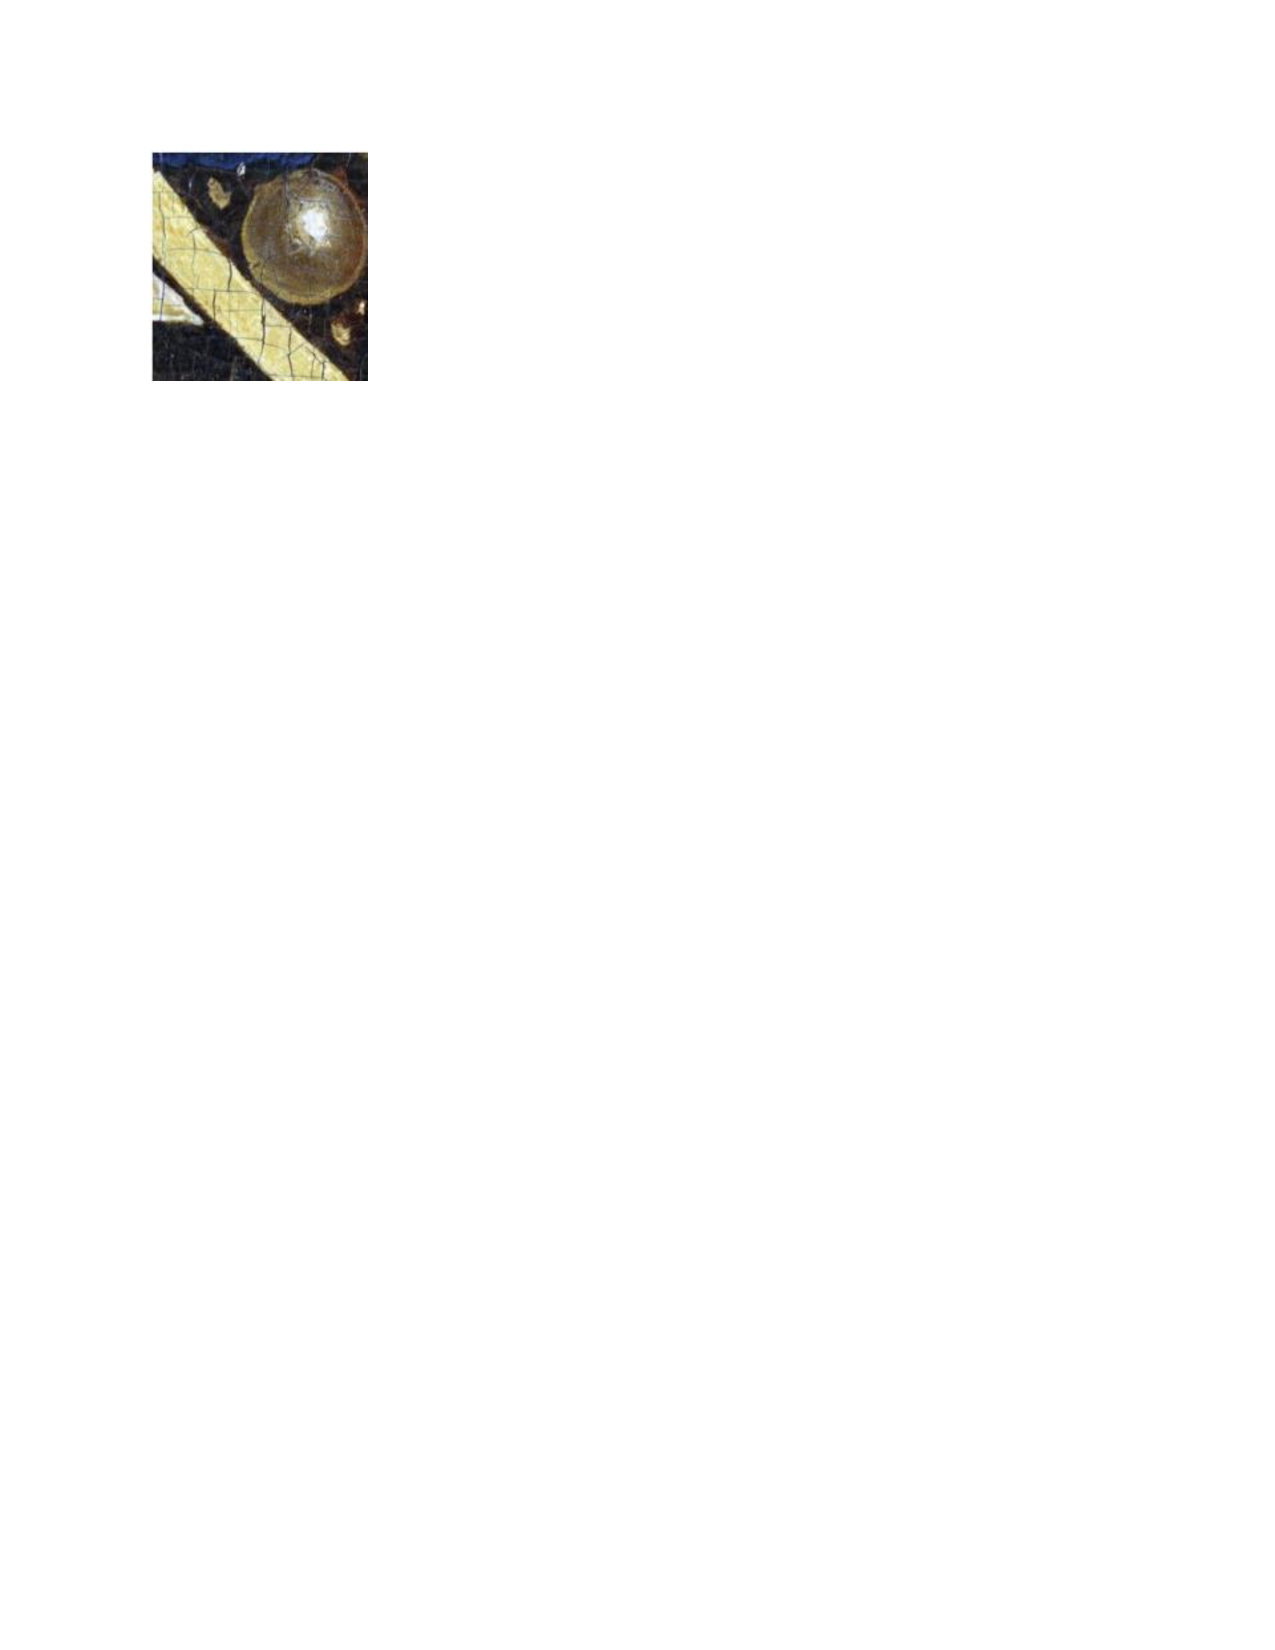
\includegraphics[width=1\textwidth,trim={0.5in 8.4in 5.5in 0.75in},clip]{ghent_altarpiece_original}
\begin{center}
{\tiny Cornelis et al}
\end{center}
\end{column}
\end{columns}
\end{frame}

\begin{frame}
  \frametitle{Outline}
  \tableofcontents[hideallsubsections]
\end{frame}

\section[Edge Detection]{Edge Detection}

\begin{frame}
\frametitle{Criteria}
Terms
\begin{description}
\item[Edge] boundaries between areas of varying intensity
\item[Intensity] brightness or dullness of a color
\end{description}
\linespace
\linespace
\begin{enumerate}
\item[1] Accuracy \ \ \ \ \ - low error rate
\item[2] Localization \ - minimal distance between detected and actual edge
\item[3] Uniqueness \ - only one response to a single edge
\end{enumerate}
\end{frame}

\begin{frame}
\frametitle{Canny Algorithm I}
\begin{columns}
\begin{column}{0.6\textwidth}
\begin{enumerate}
\item[1] Smooth image.
\item[2] Find jumps in intensity.
\item[3] Search regions for local maximum.
\end{enumerate}
\end{column}
\begin{column}{0.4\textwidth}
\begin{center}
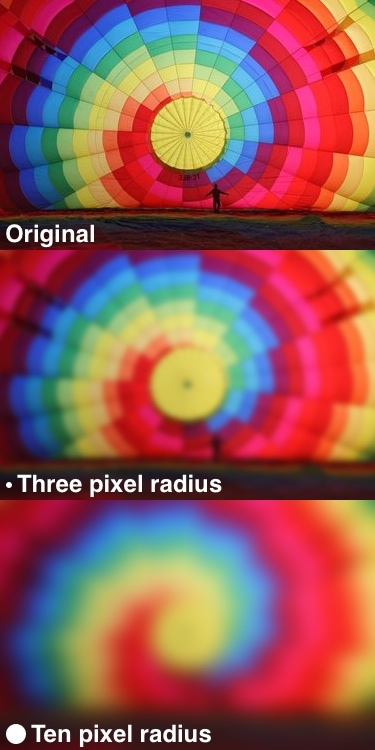
\includegraphics[width=0.65\textwidth]{gaussian_blur_example}
\linebreak
{\tiny Wikipedia}
\end{center}
\end{column}
\end{columns}
\end{frame}

\begin{frame}
\frametitle{Canny Algorithm II}
\begin{enumerate}
\item[4] Compare intensity of remaining pixels to thresholds.
\end{enumerate}
\begin{columns}
\begin{column}{0.5\textwidth}
Original Image
\begin{center}
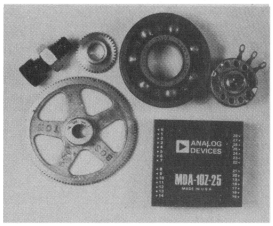
\includegraphics[width=1\textwidth]{before_edge_detection}
\linebreak
{\tiny Canny}
\end{center}
\end{column}
\begin{column}{0.5\textwidth}
Edge Mask
\begin{center}
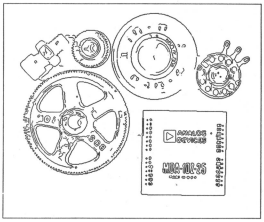
\includegraphics[width=1\textwidth]{after_edge_detection}
\linebreak
{\tiny Canny}
\end{center}
\end{column}
\end{columns}
\end{frame}

\section[Morphological Operations]{Morphological Operations}

\begin{frame}
\frametitle{Morphological Operations}
\begin{columns}
\begin{column}{0.5\textwidth}
Binary and Greyscale Images
\linebreak
\linebreak
Two Inputs:
\begin{itemize}
\item Original Image
\item Structuring Element
\end{itemize}
\end{column}
\begin{column}{0.5\textwidth}
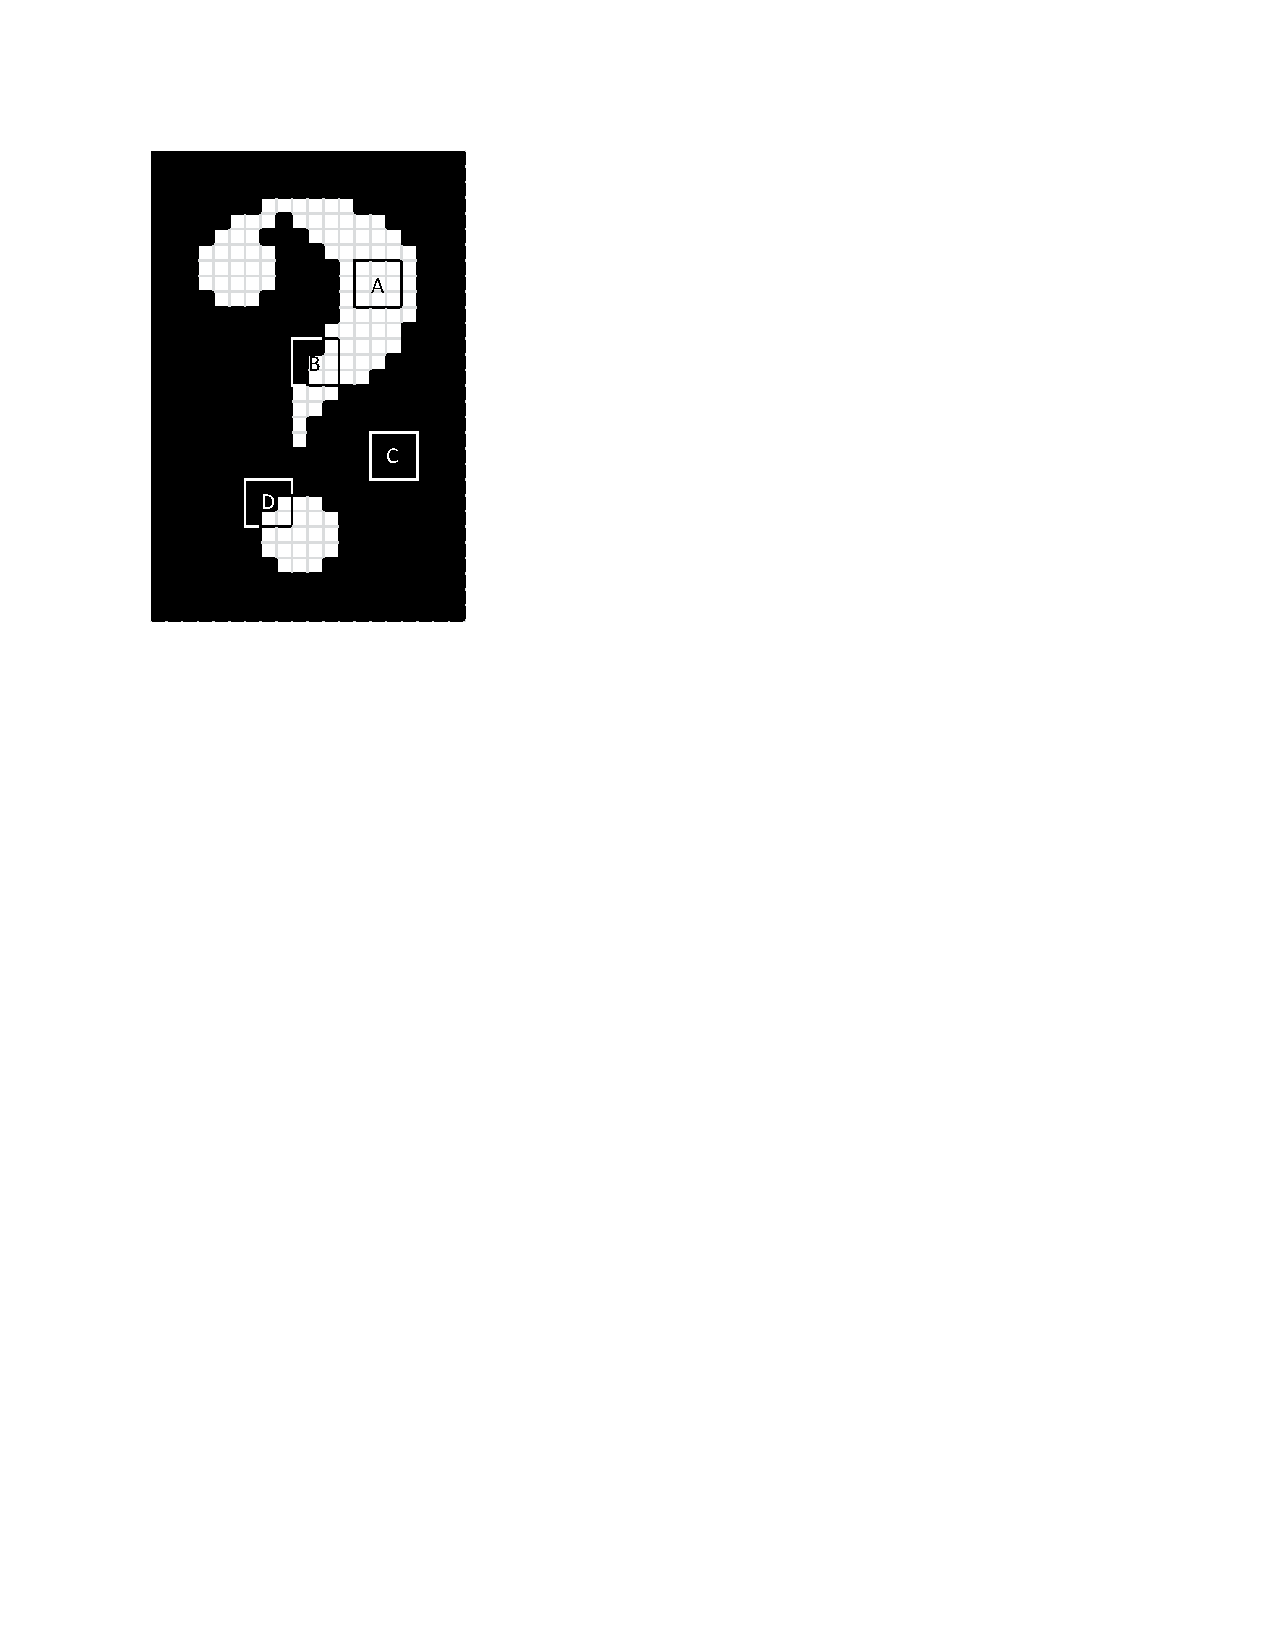
\includegraphics[width=1\textwidth,trim={0 6.5in 4in 0},clip]{structuring_element_placement}
\end{column}
\end{columns}
\end{frame}

\subsection[Erosion]{Erosion}

\begin{frame}
\frametitle{Erosion}
\begin{center}
Erosion removes foreground pixels.
\begin{equation*}
g = f \ominus s
\end{equation*}
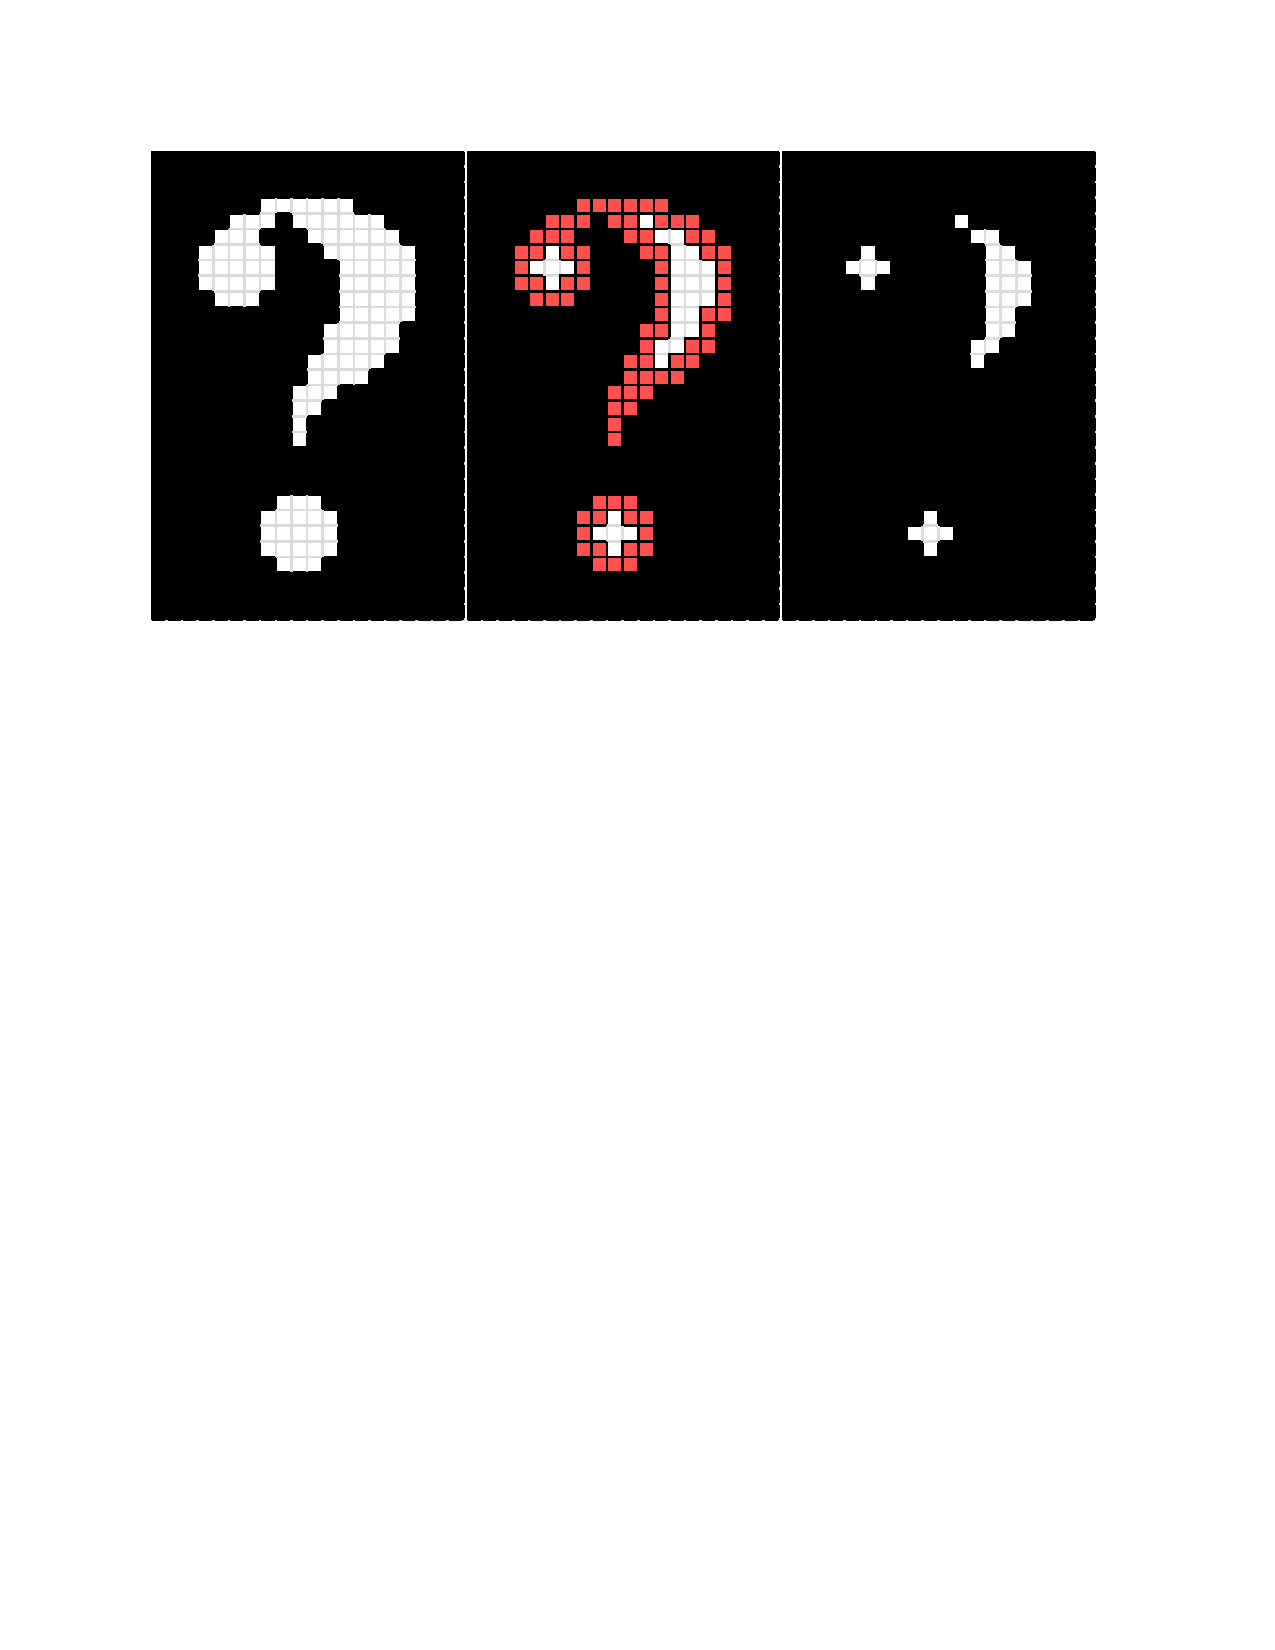
\includegraphics[width=1\textwidth,trim={0 0 0 0.5in},clip]{erosion}
\end{center}
\end{frame}

\subsection[Dilation]{Dilation}

\begin{frame}
\frametitle{Dilation}
\begin{center}
Dilation adds foreground pixels.
\begin{equation*}
g = f \oplus s
\end{equation*}

\includegraphics[width=1\textwidth,trim={0 0 0 0.5in},clip]{dilation}
\end{center}
\end{frame}

\subsection[Opening]{Opening}

\begin{frame}
\frametitle{Opening}
\begin{center}
Opening removes foreground pixels... neatly.
\begin{equation*}
g = f \circ s = (f \ominus s) \oplus s
\end{equation*}
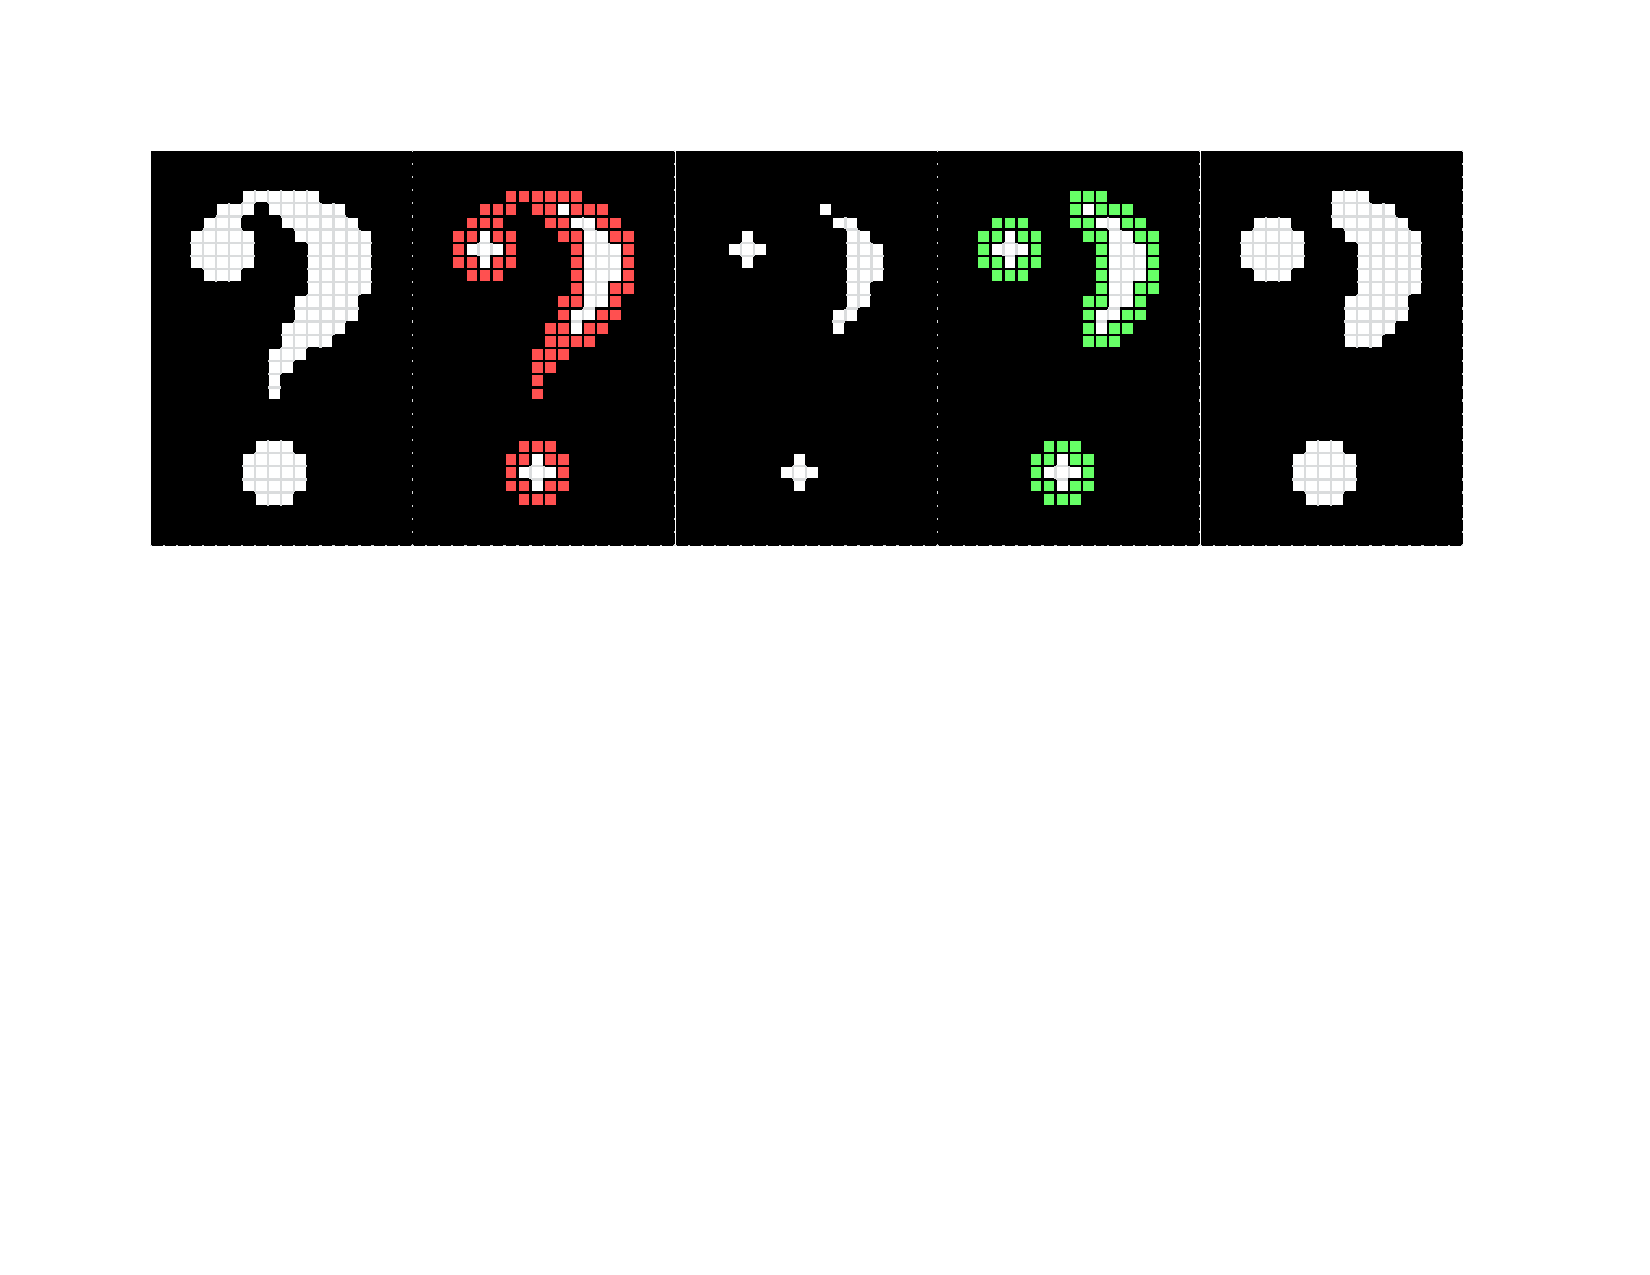
\includegraphics[width=1\textwidth,trim={0 0 0 0.5in},clip]{opening}
\end{center}
\end{frame}

\subsection[Closing]{Closing}

\begin{frame}
\frametitle{Closing}
\begin{center}
Closing adds foreground pixels... neatly.
\begin{equation*}
g = f \bullet s = (f \oplus s) \ominus s
\end{equation*}

\includegraphics[width=1\textwidth,trim={0 0 0 0.5in},clip]{closing}
\end{center}
\end{frame}

\section[Methods of Crack Detection]{Methods of Crack Detection}

\subsection[Top-Hat Transform]{Top-Hat Transform}

\begin{frame}
\frametitle{Top-Hat Algorithm}
\begin{columns}
\begin{column}{0.5\textwidth}
\begin{description}
\item[Black Top-Hat] \hfill \\ darker details on lighter background
\end{description}
\begin{equation*}
BTH = (f \bullet s) - f
\end{equation*}
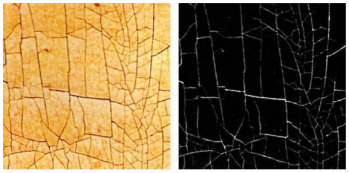
\includegraphics[width=1\textwidth]{black_top_hat}
\begin{center}
{\tiny Spagnolo and Somma}
\end{center}
\end{column}
\begin{column}{0.5\textwidth}
\begin{description}
\item[White Top-Hat] \hfill \\ lighter details on darker background
\end{description}
\begin{equation*}
WTH = f - (f \circ s)
\end{equation*}
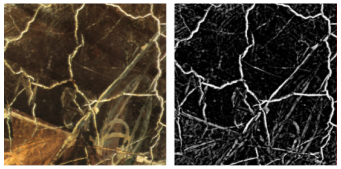
\includegraphics[width=1\textwidth]{white_top_hat}
\begin{center}
{\tiny Spagnolo and Somma}
\end{center}
\end{column}
\end{columns}
\end{frame}

\subsection[Alternative Method]{Alternative Method}

\begin{frame}
\frametitle{Alternative Method I}
\begin{columns}
\begin{column}{0.5\textwidth}
\begin{enumerate}
\item[1] Compare pixels to threshold.
\item[2] Apply closing.
\end{enumerate}
\end{column}
\begin{column}{0.5\textwidth}
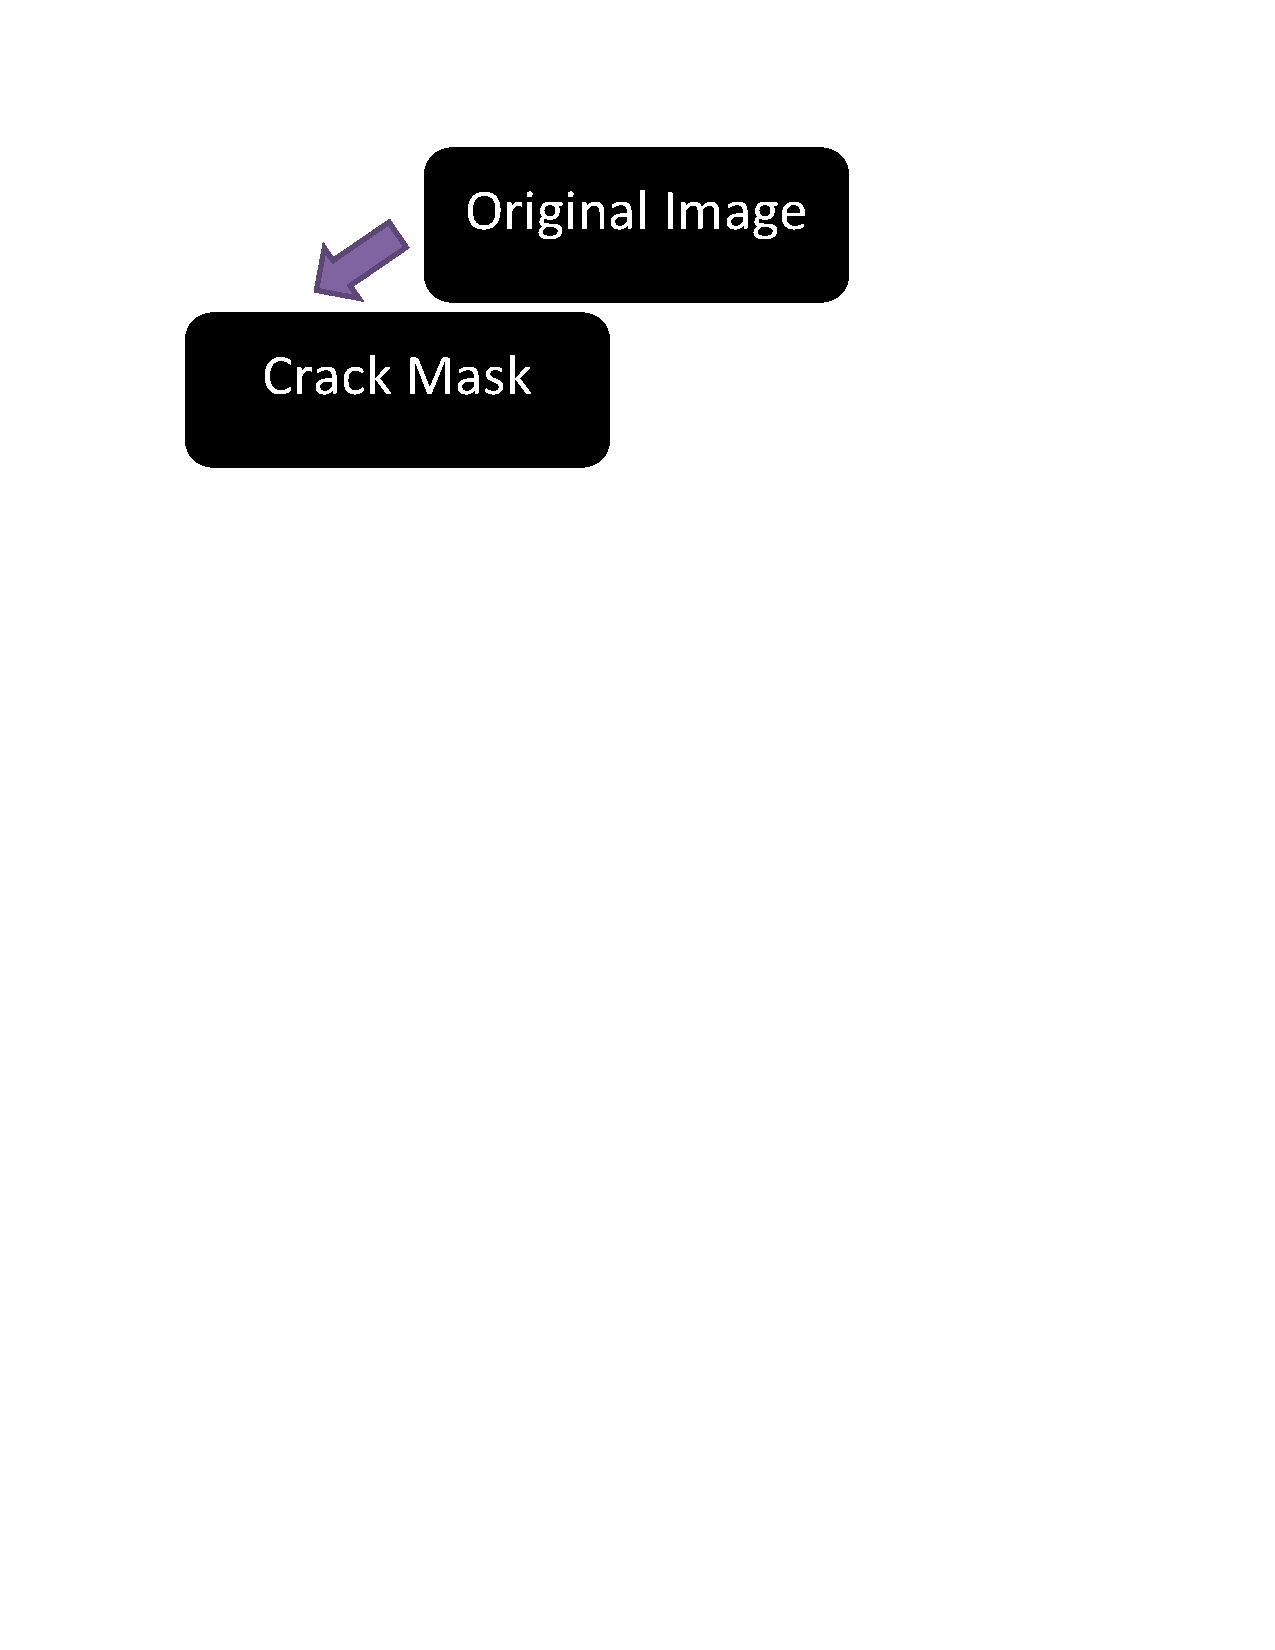
\includegraphics[width=1\textwidth,trim={1in 7.5in 2.5in 0in},clip]{alternative_method_diagram_1}
\end{column}
\end{columns}
\end{frame}

\begin{frame}
\frametitle{Alternative Method II}
\begin{columns}
\begin{column}{0.5\textwidth}
\begin{enumerate}
\item[3] Apply edge detection.
\item[4] Apply dilation.
\end{enumerate}
\end{column}
\begin{column}{0.5\textwidth}
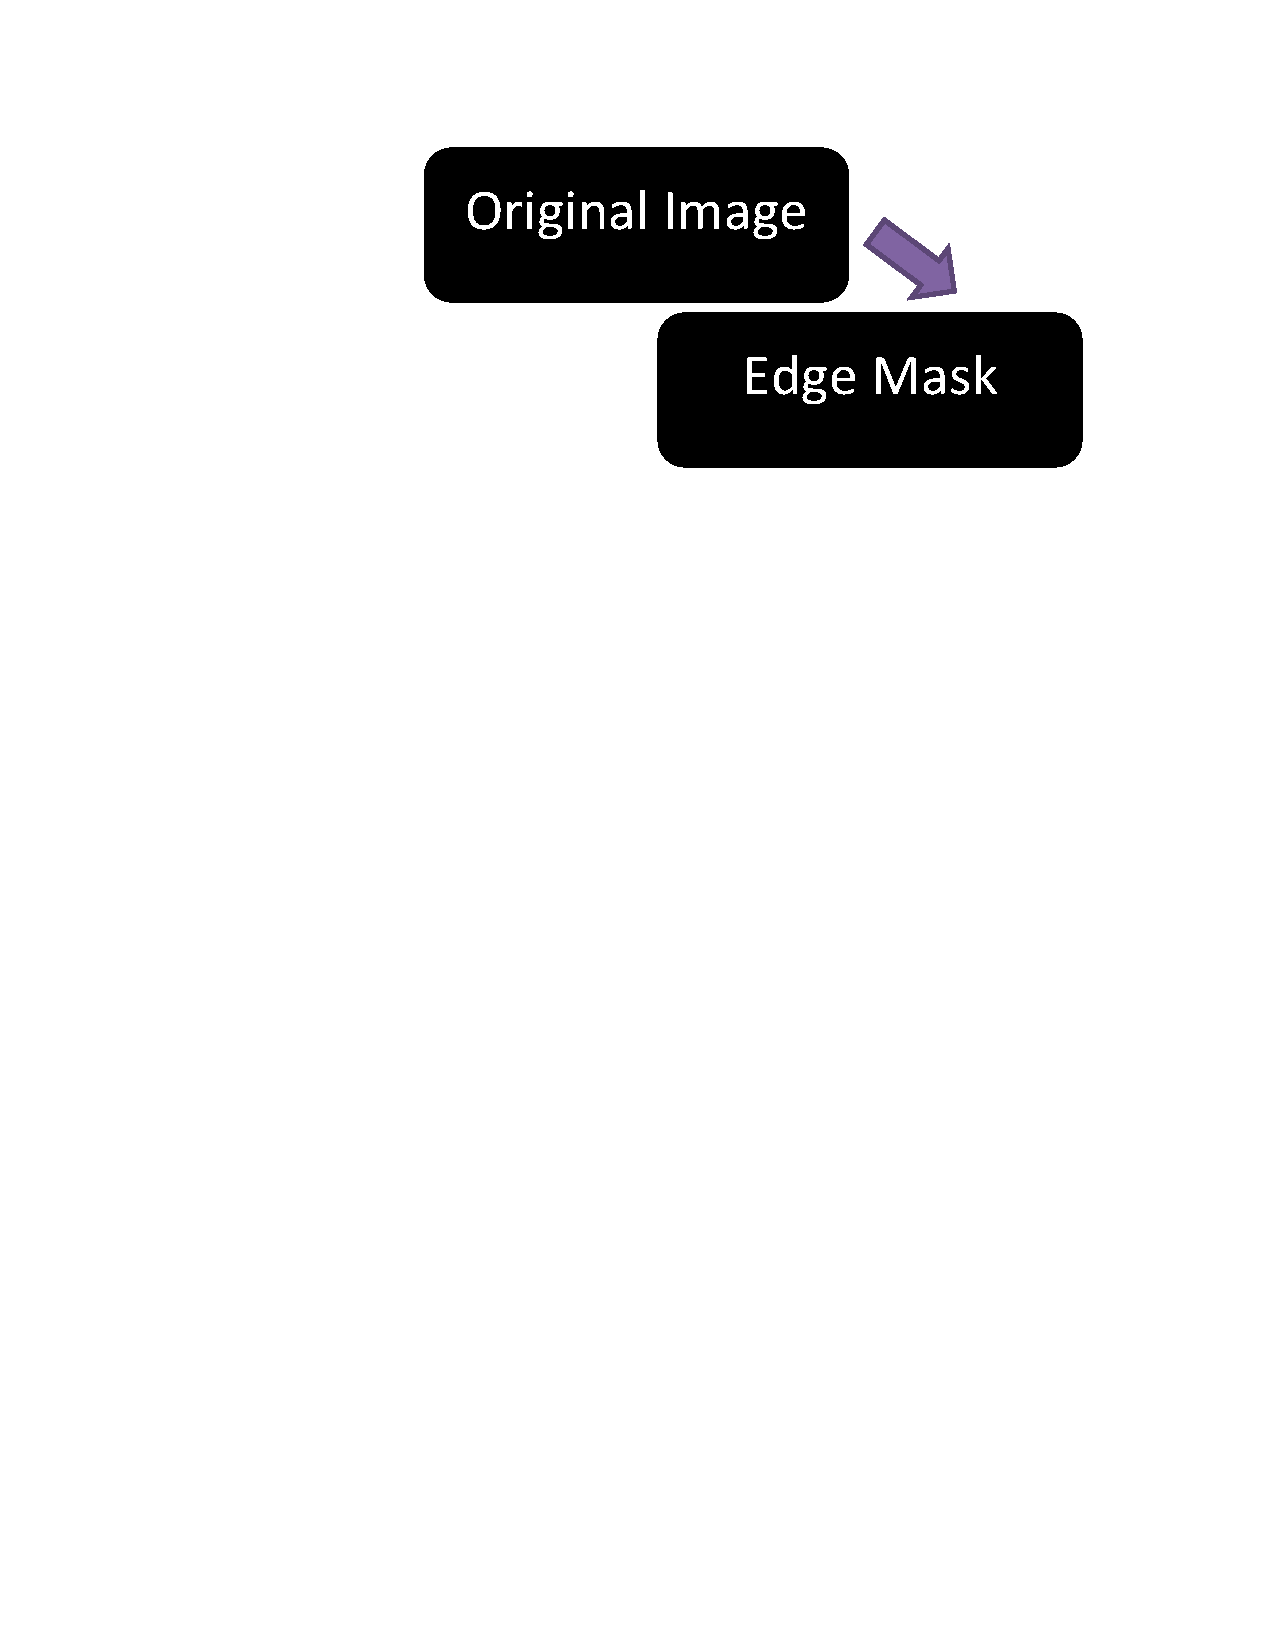
\includegraphics[width=1\textwidth,trim={2.5in 7.5in 1in 0in},clip]{alternative_method_diagram_2}
\end{column}
\end{columns}
\end{frame}

\begin{frame}
\frametitle{Alternative Method III}
\begin{columns}
\begin{column}{0.5\textwidth}
\begin{enumerate}
\item[5] Join to form binary mask.
\item[6] Apply erosion.
\end{enumerate}
\end{column}
\begin{column}{0.5\textwidth}
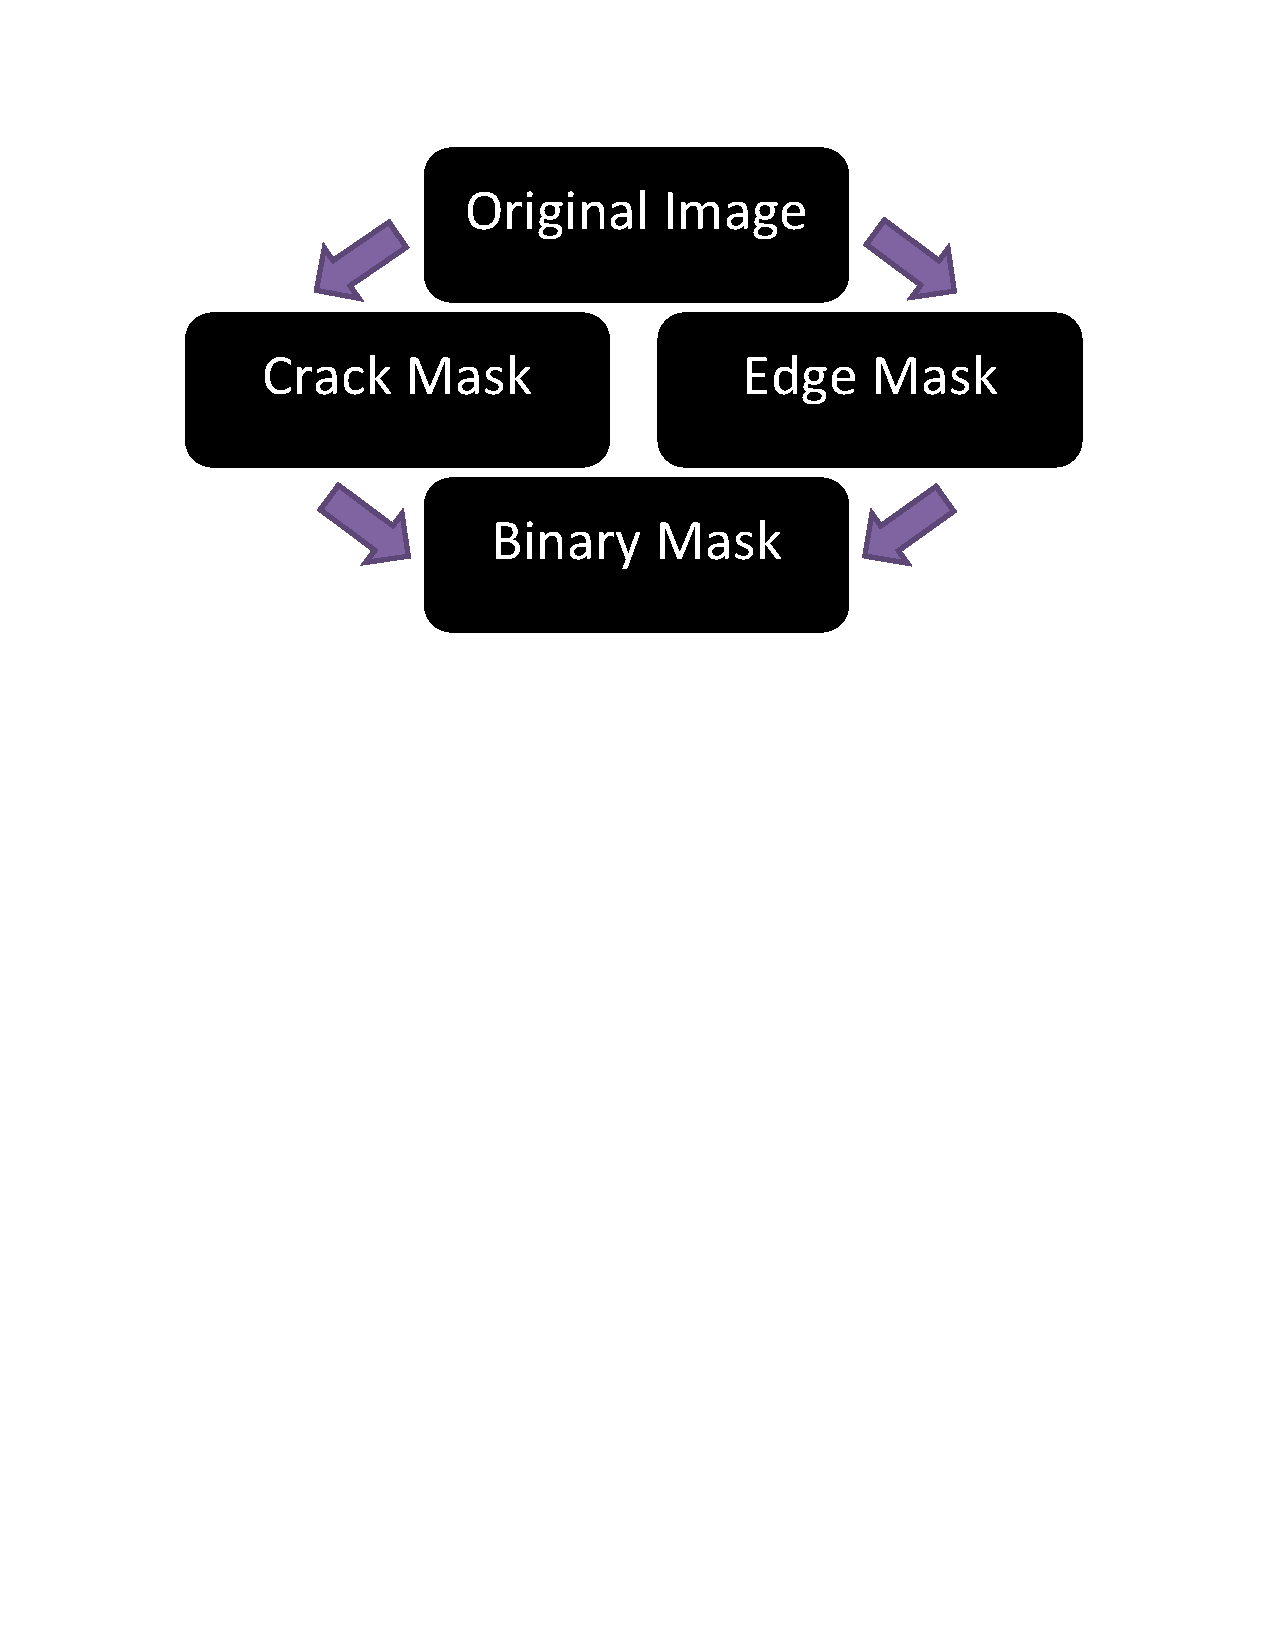
\includegraphics[width=1\textwidth,trim={1in 6.5in 1in 0in},clip]{alternative_method_diagram_3}
\end{column}
\end{columns}
\end{frame}

\section[Inpainting]{Inpainting}

\begin{frame}
\frametitle{Inpainting Process I}
\begin{columns}
\begin{column}{0.5\textwidth}
The image is broken down.
\end{column}
\begin{column}{0.5\textwidth}
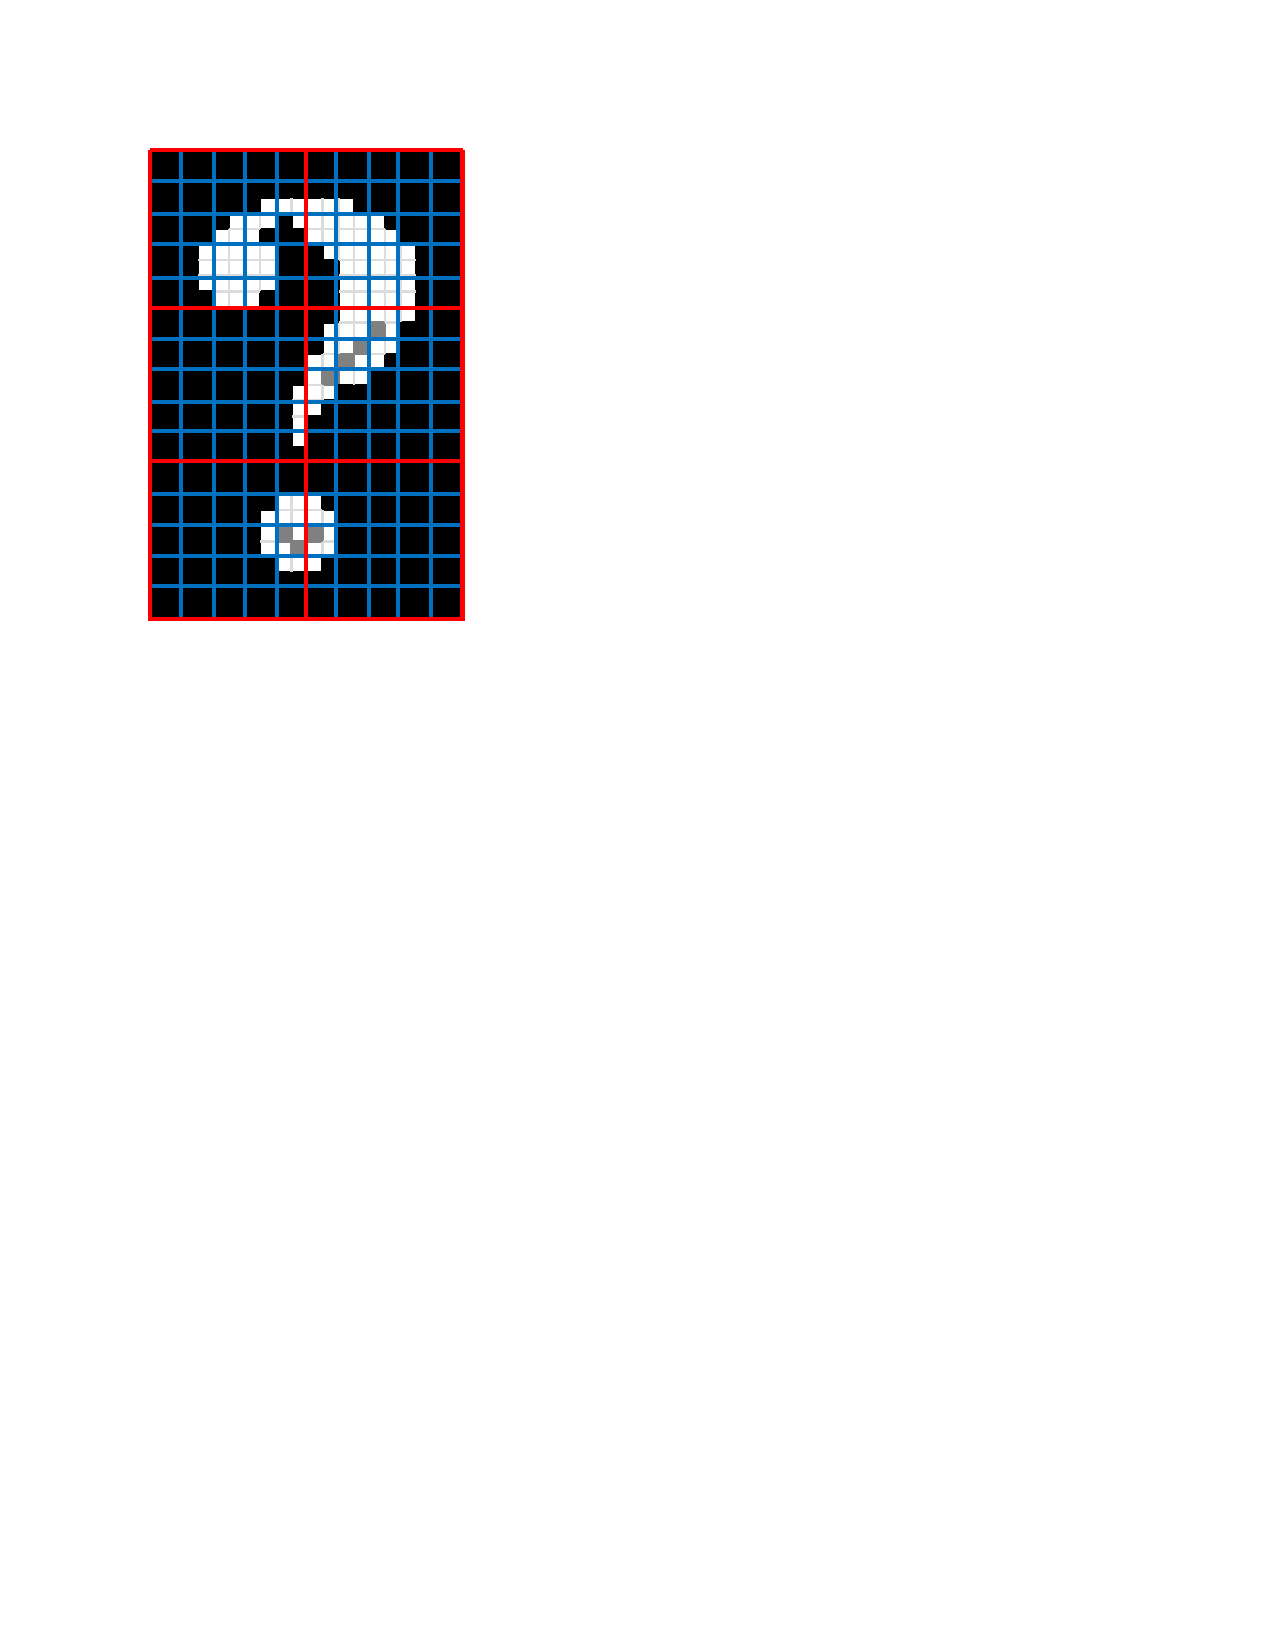
\includegraphics[width=1\textwidth,trim={0 6.5in 4in 0},clip]{regions_and_neighborhoods}
\end{column}
\end{columns}
\end{frame}

\begin{frame}
\frametitle{Inpainting Process II}
\begin{columns}
\begin{column}{0.5\textwidth}
For each defective pixel $i$:
\begin{enumerate}
\item[1] Find the context of $i$.
\item[2] Find most similar neighborhood in region.
\end{enumerate}
\end{column}
\begin{column}{0.5\textwidth}
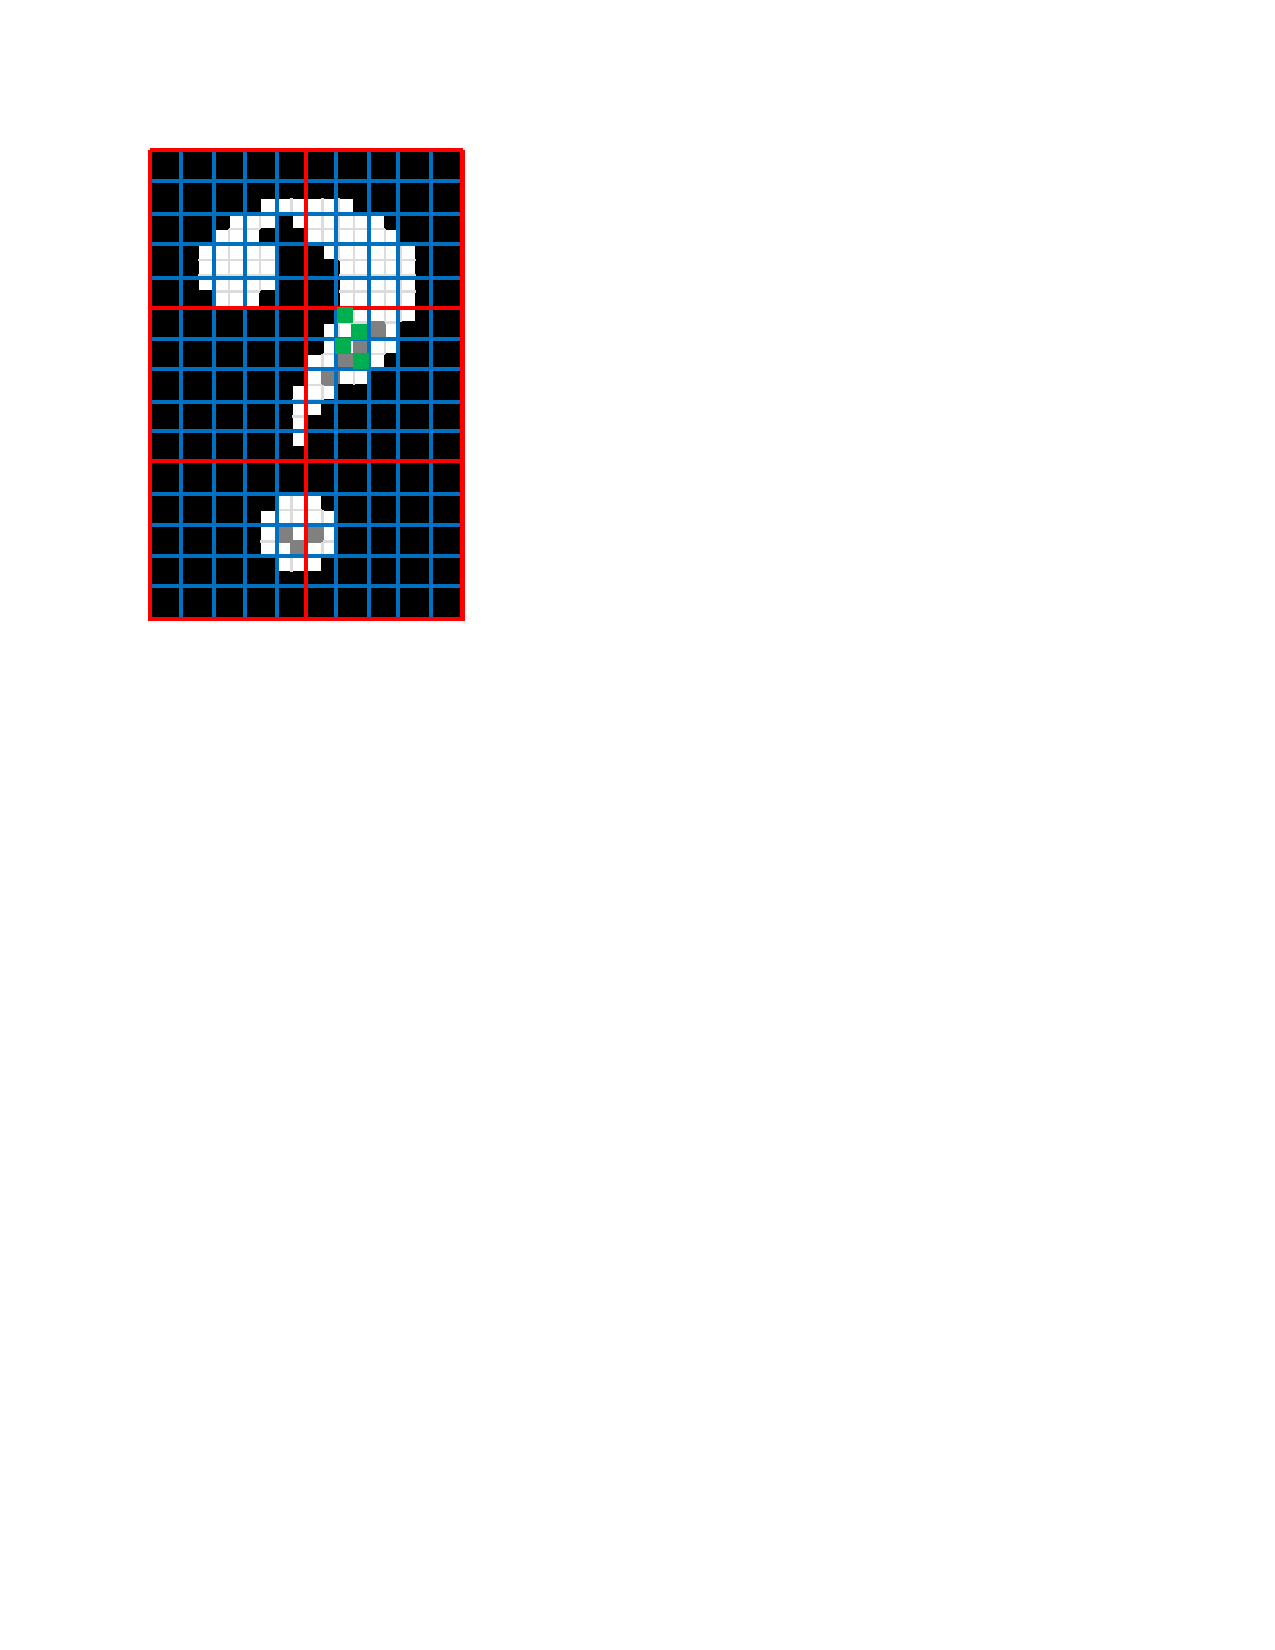
\includegraphics[width=1\textwidth,trim={0 6.5in 4in 0},clip]{context_and_match}
\end{column}
\end{columns}
\end{frame}

\begin{frame}
\frametitle{Inpainting Process III}
\begin{columns}
\begin{column}{0.45\textwidth}
\begin{enumerate}
\item[3] Replace all defective pixels in the neighborhood of $i$ with corresponding pixels from most similar neighborhood.
\end{enumerate}

\end{column}
\begin{column}{0.1\textwidth}
OR
\end{column}
\begin{column}{0.45\textwidth}
\begin{enumerate}
\item[3] Replace pixel $i$ with the median value of all non-defective pixels within its neighborhood.
\end{enumerate}

\end{column}
\end{columns}
\begin{columns}
\begin{column}{0.45\textwidth}
\begin{center}
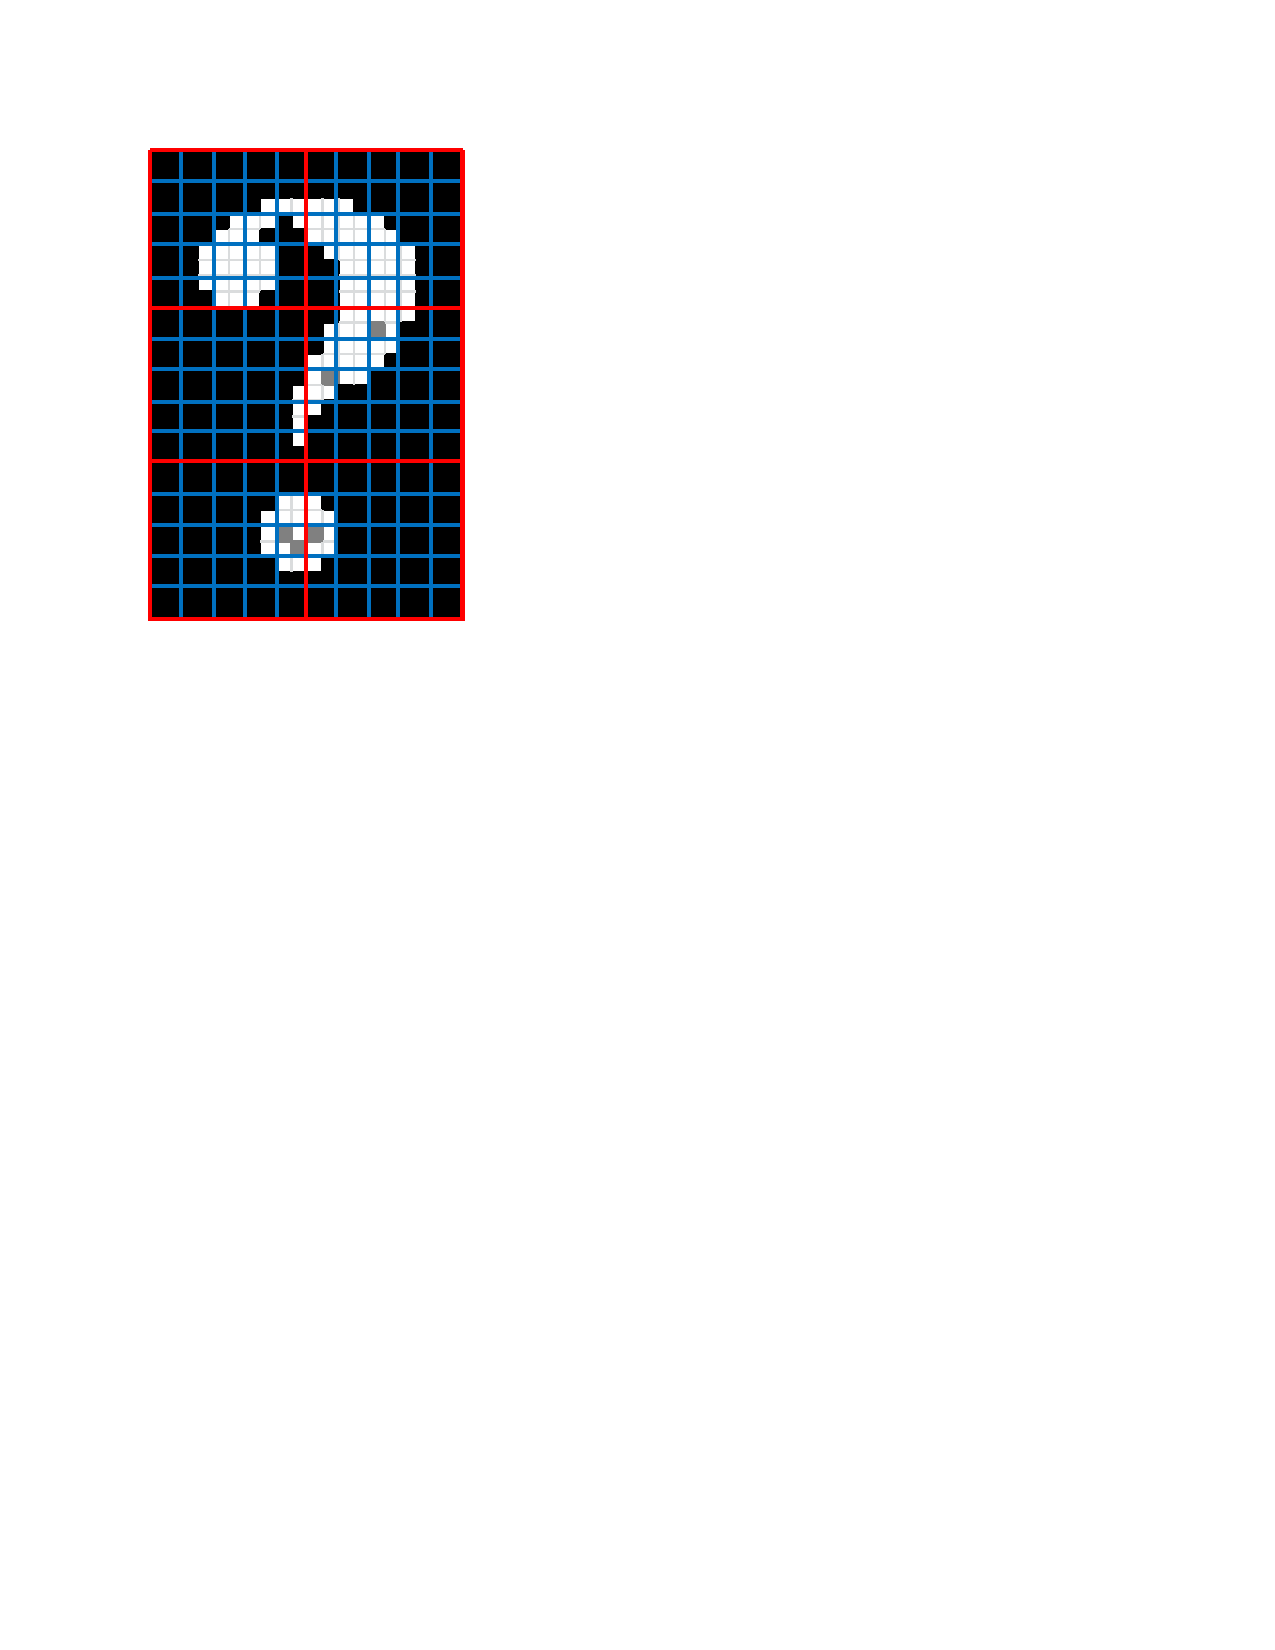
\includegraphics[width=1\textwidth,trim={0 6.5in 4in 1in},clip]{replace_defect_1}
\end{center}
\end{column}
\begin{column}{0.1\textwidth}
\end{column}
\begin{column}{0.45\textwidth}
\begin{center}
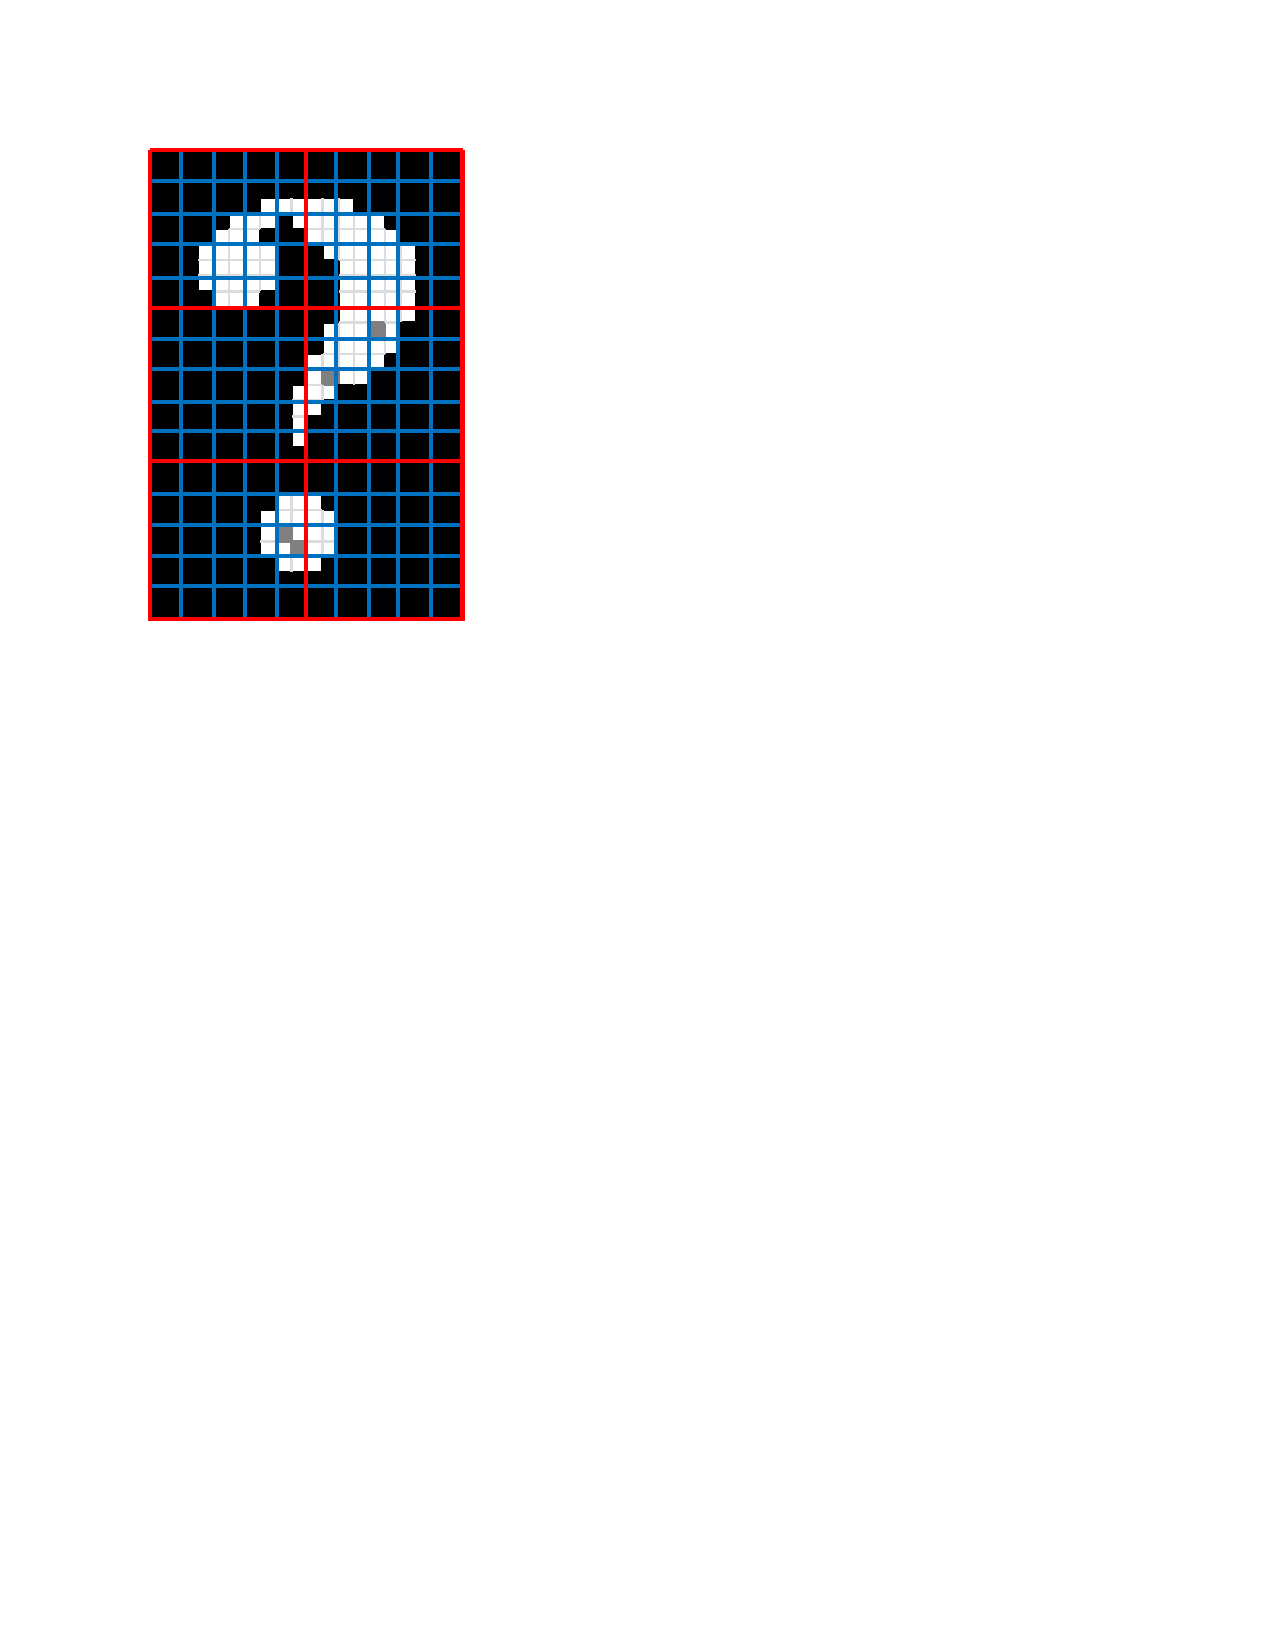
\includegraphics[width=1\textwidth,trim={0 6.5in 4in 1in},clip]{replace_defect_2}
\end{center}
\end{column}
\end{columns}
\end{frame}

\section[Results]{Results}

\begin{frame}
\frametitle[Definitions]{Definitions}
\begin{center}
Categories:
\end{center}
{\footnotesize
\begin{itemize}
\item true positives (\textit{tp})
\item false positives (\textit{fp})
\item true negatives (\textit{tn})
\item false negatives (\textit{fn})
\end{itemize}
}
\begin{center}
Equations:
\end{center}
\begin{columns}
\begin{column}{0.5\textwidth}
{\footnotesize
False and True Positive Rate
\begin{equation*}
FP = fp / (fp + tn)
\end{equation*}
\begin{equation*}
TP = tp / (tp + fn)
\end{equation*}
}
\end{column}
\begin{column}{0.5\textwidth}
{\footnotesize
Precision and Recall
\begin{equation*}
P = tp / (tp + fp)
\end{equation*}
\begin{equation*}
R = tp / (tp + fn)
\end{equation*}
}
\end{column}
\end{columns}
\end{frame}

\begin{frame}
\frametitle[Statistics]{Statistics I}
\begin{table}
\centering
\resizebox{10cm}{!}{
\begin{tabular}{|l|l|r|r|r|r|r|r|r|}
\hline
\textbf{Method} & \textbf{Classification} & \textbf{\textit{tp}} & \textbf{\textit{fn}} & \textbf{\textit{tn}} & \textbf{\textit{fp}} & \textbf{\textit{TP} (or \textit{R})} & \textbf{\textit{FP}} & \textbf{\textit{P}}\\ \hline
\multirow{8}{*}{Top-Hat Transform}
& Crack Thickness - Thin & 220 & 30 & 230 & 20 & 0.880 & 0.080 & 0.917\\ \cline{2-9}
& Crack Thickness - Medium & 232 & 18 & 231 & 19 & 0.928 & 0.076 & 0.924\\ \cline{2-9}
& Crack Thickness - Thick & 235 & 15 & 238 & 12 & 0.940 & 0.048 & 0.951\\ \cline{2-9}
& Number of Cracks - Few & 242 & 8 & 245 & 5 & 0.968 & \textbf{0.020} & 0.980\\ \cline{2-9}
& Number of Cracks - Medium & 245 & 5 & 241 & 9 & \textbf{0.980} & 0.036 & 0.965\\ \cline{2-9}
& Number of Cracks - Many & 243 & 7 & 243 & 7 & 0.972 & 0.028 & 0.972\\ \cline{2-9}
& Crack Connectivity - Low & 215 & 35 & 219 & 31 & \textbf{0.860} & \textbf{0.124} & 0.874\\ \cline{2-9}
& Crack Connectivity - High & 218 & 32 & 221 & 29 & 0.872 & 0.116 & 0.883\\ \hline
\multirow{3}{*}{Alternative Method}
& Edge Information Lost - 1\% & - & - & - & - & \textbf{0.932} & - & \textbf{0.497}\\ \cline{2-9}
& Edge Information Lost - 30\% & - & - & - & - & 0.857 & - & 0.594\\ \cline{2-9}
& Edge Information Lost - 70\% & - & - & - & - & \textbf{0.530} & - & \textbf{0.704}\\ \hline
\end{tabular}
}
\end{table}
\end{frame}

\begin{frame}
\frametitle{Statistics II}
\begin{center}
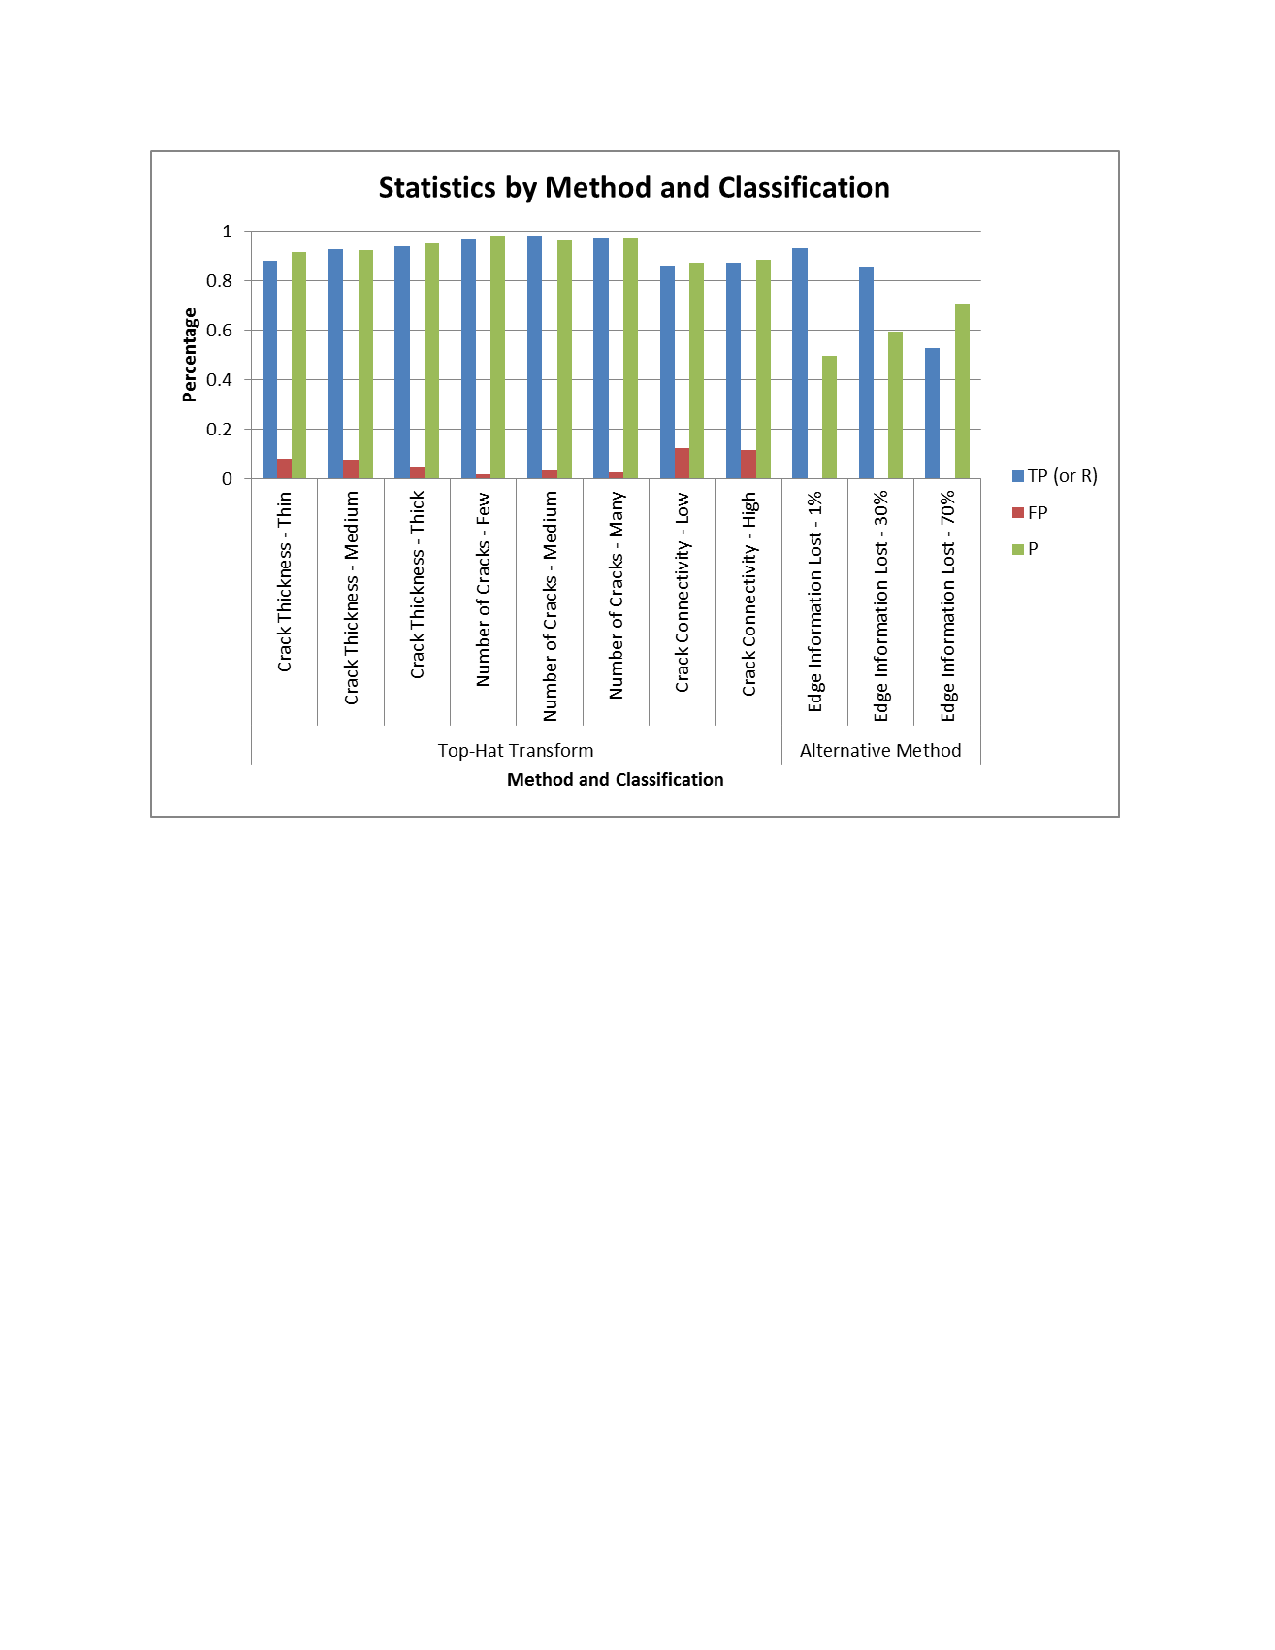
\includegraphics[width=0.8\textwidth,trim={1in 5in 1in 1in},clip]{results_graph}
\end{center}
\end{frame}

\begin{frame}
\frametitle[Results]{Results}
\begin{columns}
\begin{column}{0.5\textwidth}
Original Image
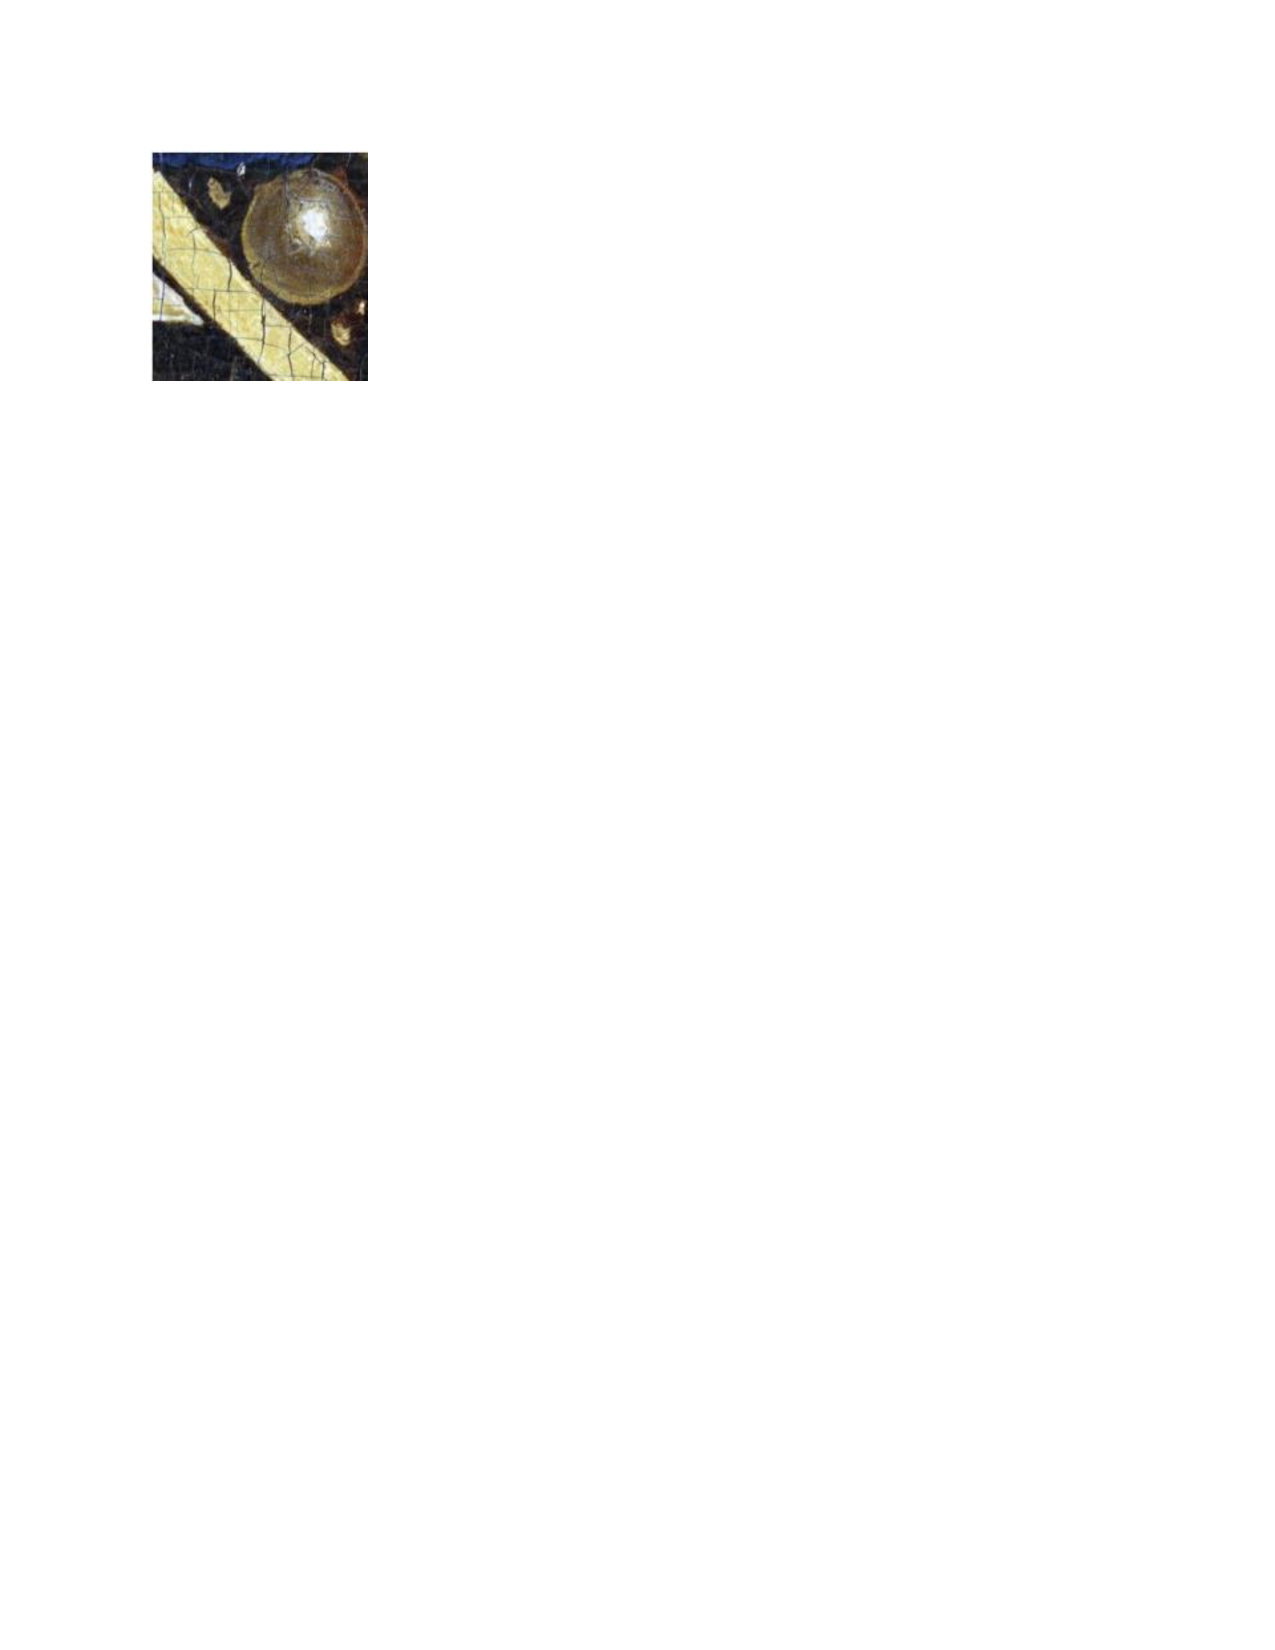
\includegraphics[width=1\textwidth,trim={0.5in 8.4in 5.5in 0.75in},clip]{ghent_altarpiece_original}
\begin{center}
{\tiny Cornelis et al}
\end{center}
\end{column}
\begin{column}{0.5\textwidth}
Restored Image
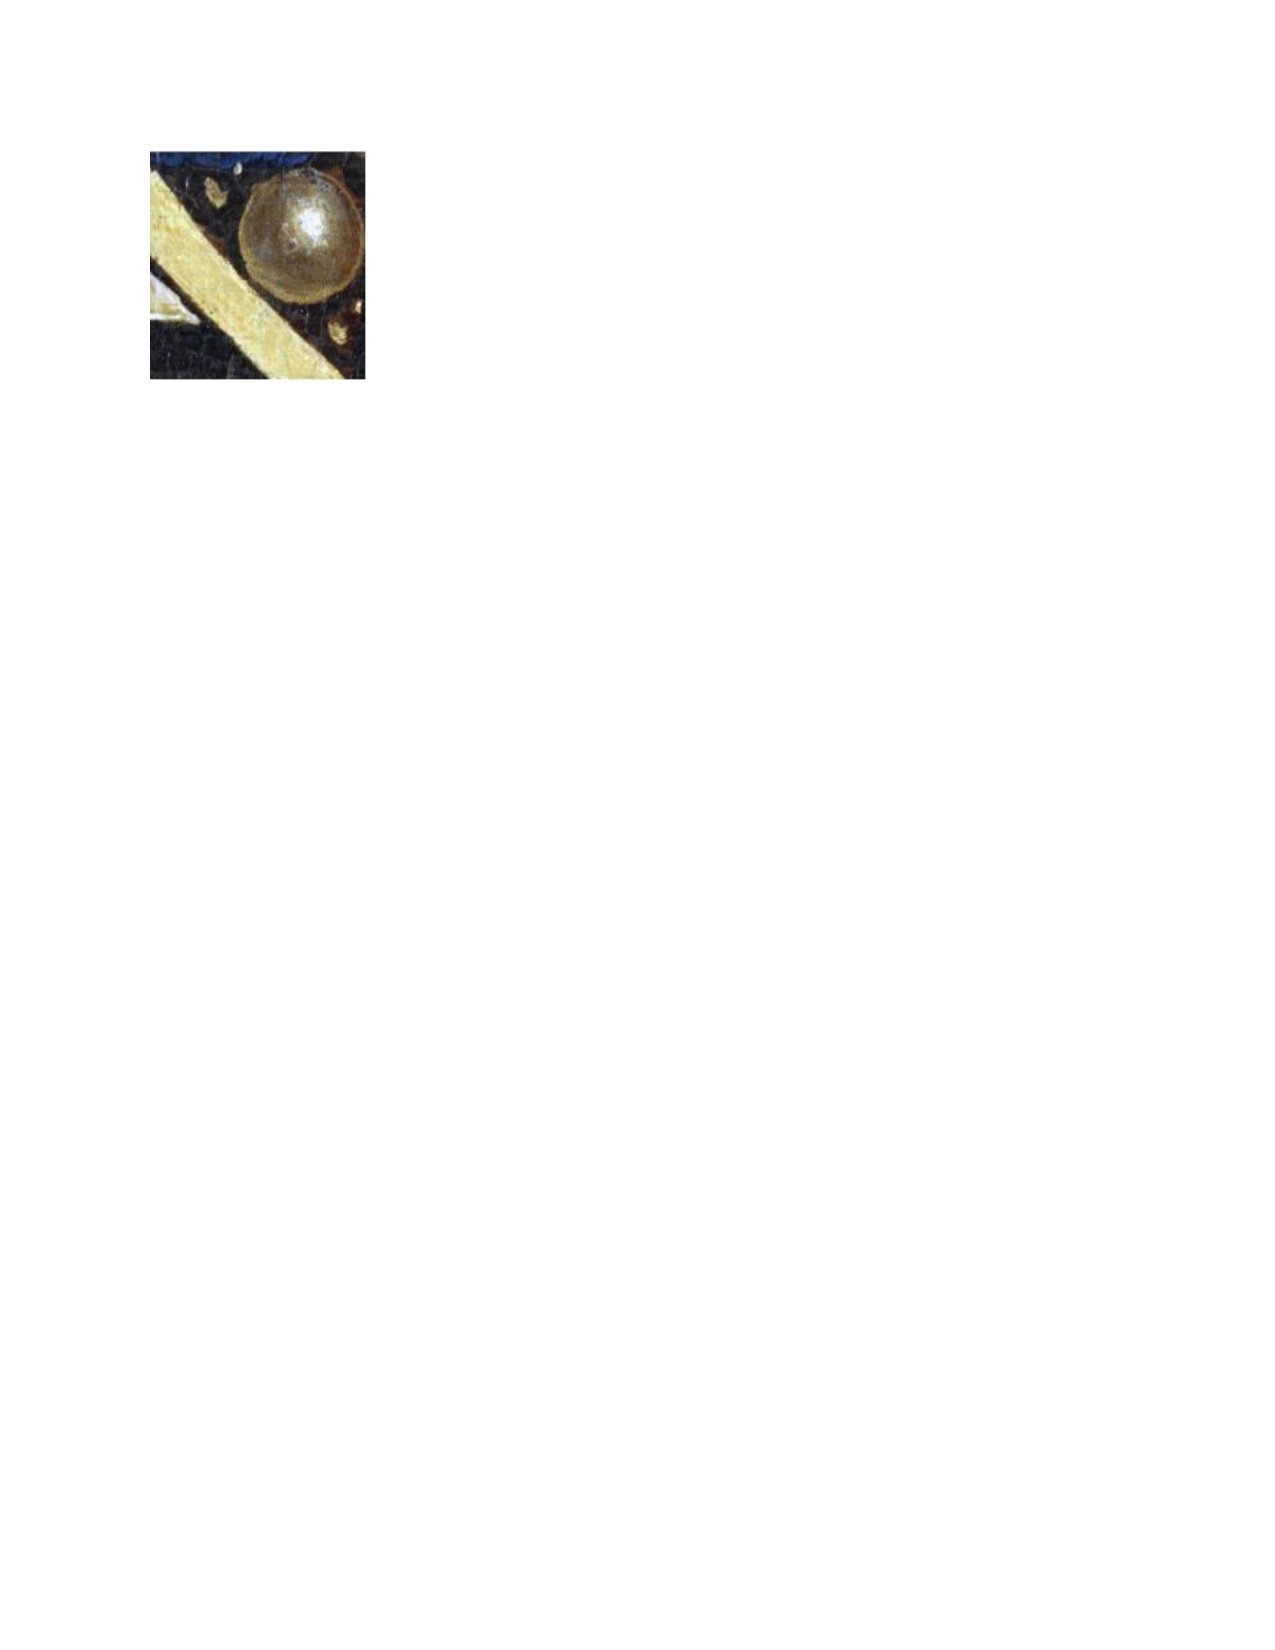
\includegraphics[width=1\textwidth,trim={0.5in 8.4in 5.5in 0.75in},clip]{ghent_altarpiece_restored}
\begin{center}
{\tiny Cornelis et al}
\end{center}
\end{column}
\end{columns}
\end{frame}

\section[Conclusions]{Conclusions}

\begin{frame}
\frametitle[Conclusions]{Conclusions}
The top-hat transform has been demonstrated to outperform the alternative examined here.
\linebreak
\linebreak
\linebreak
Further Work:
\begin{itemize}
\item Implement other methods of crack detection.
\item Examine effects of various forms of edge detection and inpainting.
\item Study the detection and removal of other defects.
\end{itemize}
\end{frame}

\begin{frame}
\frametitle{Thanks!}
\linespace
\linespace
%Contact: \texttt{dramd002@morris.umn.edu}
\linespace
\linespace
\begin{center}
{\huge Questions?}
\end{center}
\end{frame}

\section*{References}

\begin{frame}[allowframebreaks] 
\frametitle{References} 
\nocite{*}
\bibliographystyle{abbrv}
{\tiny \bibliography{paper}}
\end{frame}

\end{document}